%\begin{figure}[!t]
%  \centering
%  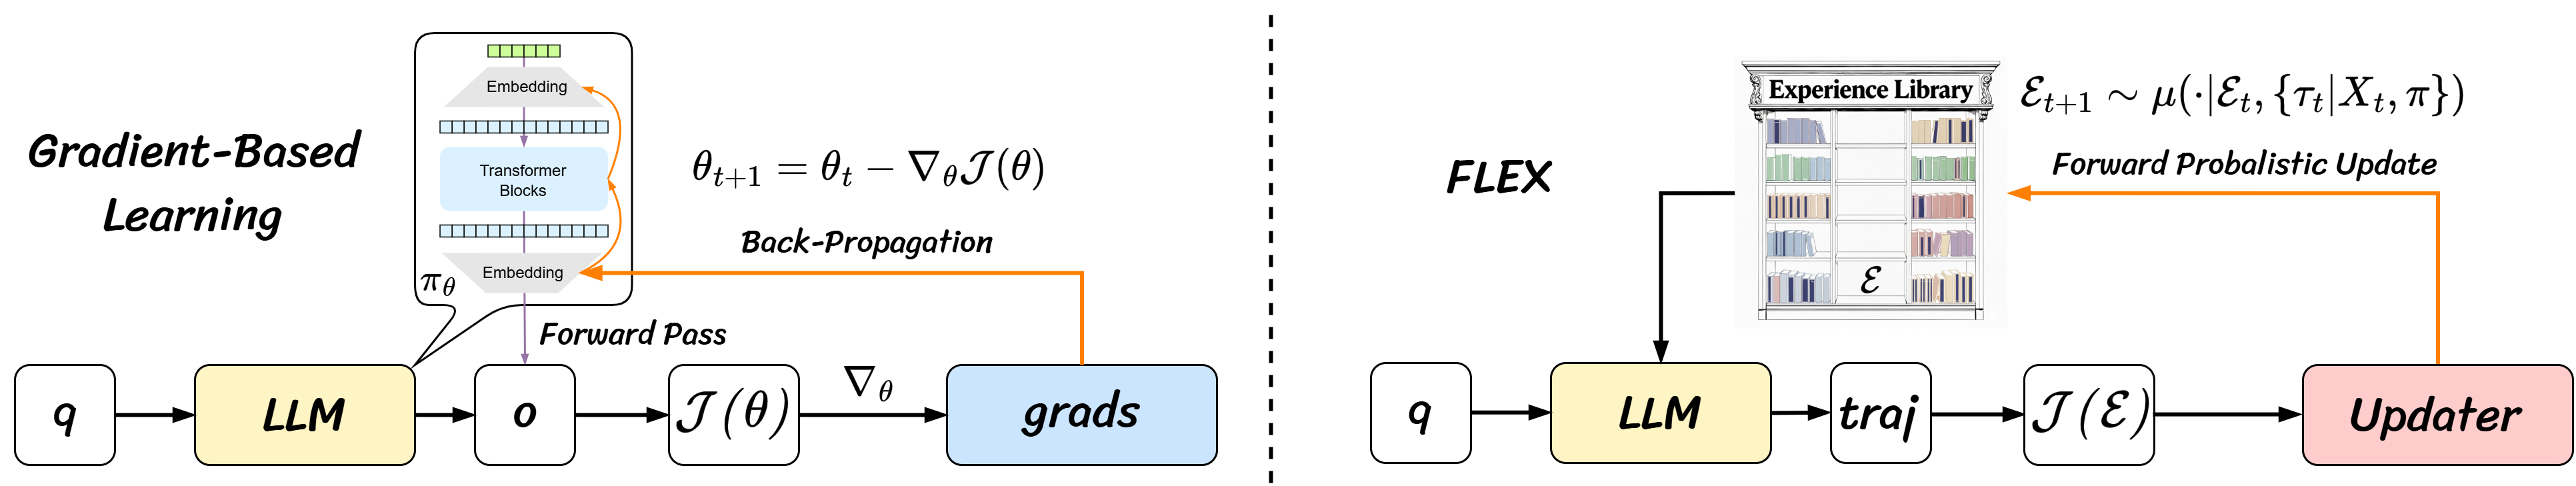
\includegraphics[width=0.95\linewidth]{./figs/method_pic.png}
%  \caption{Conceptual comparison between gradient-based learning and \method{}. Traditional gradient-base learning update parameters through backward gradient propagation, while \method{} evolves the experience library via forward probabilistic update, enabling continuous enhancement without parameter updates.}
%  \label{fig:method_pic}
%\end{figure}
%\clearpage
\section{Forward Learning with Experience}
In this section, we establish a unified mathematical formulation of \method{} paradigm. 
A learning paradigm typically consists of two key components: an \emph{optimization objective} (defining \textit{what} to learn) and an \emph{optimization process} (defining \textit{how} to learn it). We next illustrate how \method{} implements these components.
%罗列本章outlines？


\subsection{Overview of \method{}}
\method{} enables LLM agents to continually evolve through \textbf{learning from experience}. 
Instead of fine-tuning model parameters, \method{} focuses on constructing an \textbf{experience library} that captures and reuses knowledge distilled from past problem-solving trajectories, guiding future reasoning.

%\method{} optimizes the experience library to distill insights and lessons from experiential interactions, enabling agents to continuously evolve with enhanced reasoning and knowledge utilization. 
\method{} paradigm introduces a forward learning loop with two interleaved phases:
(i) extensive \textit{forward} exploration by the actor to collect and distill new experiences, which are integrated into the library by the updater; 
(ii) utilizing the most pertinent experiences to guide \textit{forward} reasoning on new tasks. 
As the experience library expands, it accumulates diverse, high-quality problem-solving strategies, allowing agents to leverage prior knowledge for increasingly superior reasoning, all without gradient-based parameter updates. 
Through this iterative process, agents continuously learn from accumulated experience, progressively enhancing their performance on challenging problems.
Fig.~\ref{fig:main_method_overview} illustrates the overall workflow of \method{}, showing the interaction between the actor $\pi$, updater $\mu$, and the experience library $\mathcal{E}$.

Specifically, the LLM agent $\pi$ remains frozen while being driven to explore the environment extensively, generating interaction trajectories $\{\tau \mid X, \pi\}$ for a given query $X$.
These trajectories are dynamically consolidated into the ever-evolving experience library $\mathcal{E}$ by an auxiliary updater agent $\mu$. 
Thus the library update can be denoted as $\mathcal{E}_{new}\sim\mu(\cdot\mid\mathcal{E}_{old},\{\tau\mid X,\pi\})$. The learned library accumulates distilled knowledge over time and subsequently serves as a guidance source for reasoning on future tasks.

At inference time, the most pertinent and helpful experiences are identified and fetched through $\varepsilon\sim\rho(\cdot\mid q,\mathcal{E})$ from the learned experience library $\mathcal{E}$ given query $q$.  
Conditioned on these retrieved experiences $\varepsilon$, $\pi$ is enabled to invoke learned strategies and latent cognitive patterns, producing superior response $\pi(\cdot \mid q, \varepsilon)$ that exhibit significantly enhanced reasoning capability and expert-level knowledge utilization compared to the base model.

Formally, we define the optimization objective of \method{} as constructing an optimal experience library $\mathcal{E^*}$ that maximizes expected correctness on training tasks, and operationalize it through a forward update process.
%Training 阶段训练目标为 构建最大化training accuracy的经验库$\mathcal{E}$
\paragraph{Optimization Objective.}
The optimization goal of \method{} is to construct an experience library that maximizes the expected correctness of the model’s outputs, thus we have:
\begin{definition}[Optimization Objective of \method{}]
\label{def:objective}
Given a training set $\mathcal{D} = \{(X_i, Y_i)\}_{i=1}^N$, where $X_i$ is a query and $Y_i$ is the corresponding ground truth, the objective function $\mathcal{J}(\mathcal{E})$ and the optimal experience library $\mathcal{E}^*$ is defined as:
%\begin{equation}
%\mathcal{J}(\mathcal{E}) = \mathbb{E}_{\begin{subarray}{l}
%(X_i,Y_i)\sim\mathcal{D},\\
%\varepsilon_i\sim\rho(\cdot\mid X_i,\mathcal{E})
%\end{subarray}}\left[\Phi (\pi(\cdot\mid X_i,\varepsilon_i), Y_i)\right],\quad \mathcal{E}^* = %\arg\max_{\mathcal{E}}\mathcal{J}(\mathcal{E})
%\label{eq:obj}
%\end{equation}
\begin{equation}
\begin{aligned}
\mathcal{J}(\mathcal{E}) 
&= \mathbb{E}_{(X_i, Y_i)\sim\mathcal{D},\, \varepsilon_i\sim\rho(\cdot\mid X_i,\mathcal{E})}
  \big[\Phi\big(\pi(\cdot\mid X_i,\varepsilon_i),\, Y_i\big)\big], \\
\mathcal{E}^* 
&= \arg\max_{\mathcal{E}}\, \mathcal{J}(\mathcal{E})
\end{aligned}
\label{eq:obj}
\end{equation}
where $\rho(\cdot\mid X_i,\mathcal{E})$ retrieves experiences $\varepsilon_i$ from library $\mathcal{E}$ given query $X_i$, $\pi(\cdot\mid X_i,\varepsilon_i)$ is the LLM agent conditioned on both the query and retrieved experiences, and $\Phi(\hat{Y}, Y_i)$ measures the correctness of prediction $\hat{Y}$ against ground truth $Y_i$.
\end{definition}
This objective serves as the guiding principle for the experience library evolution in \method{}, explicitly linking the quality of the experience library to the model's ultimate performance on target tasks.

%我们有了objective，现在我们来分析objective如何指导learning的过程。对于传统gradient-based方法，学习过程是对objective梯度，接着反向传播梯度，更新参数。而forward learning的本质是用一个前向的概率分布更新experience library，替代掉了反向的梯度更新，从而实现experience library的不断evolving优化。所以我们可以类比的定义forward learning的学习更新为：dL/de \approx \rho(e_i+1|x_i, y_i, e_i)。
\paragraph{Optimization Process.}
\method{} operationalizes the objective in Definition~\ref{def:objective} through a forward learning process. 
Instead of relying on gradient-based parameter updates, learning occurs via forward probabilistic updates to the experience library, carried out by the updater agent $\mu$.
This process distills knowledge from interaction trajectories generated by $\pi$, steering the experience library toward optimization of the objective function. 
Therefore, the learning update rule for \method{} can be analogously defined as follows:

\begin{definition}[Update Rule of \method{}]
\label{def:forward_update}
The learning process in \method{} is governed by a forward update rule that evolves the experience library through forward probabilistic updates with experiential exploration, defined as:
%\begin{equation}
%\mathcal{E}_{i+1}\sim\mu(\cdot\mid\mathcal{E}_{i},\{\tau_i|X_i,\pi\}),\quad %\nabla_{\mathcal{E}}\mathcal{J}(\mathcal{E}_i)\triangleq\mu(\cdot\mid\mathcal{E}_{i},\{\tau_i|X_i,\pi\})\setminus\mathcal{E}_{i}
%\end{equation}
\begin{equation}
\begin{aligned}
\mathcal{E}_{i+1} 
&\sim \mu\big(\cdot \,\mid\, \mathcal{E}_i, \{\tau_i \mid X_i, \pi\}\big), \\
\nabla_{\mathcal{E}}\mathcal{J}(\mathcal{E}_i) 
&\triangleq \mu\big(\cdot \,\mid\, \mathcal{E}_i, \{\tau_i \mid X_i, \pi\}\big) - \mathcal{E}_i
\end{aligned}
\label{eq:meta_update}
\end{equation}
where $\{\tau_i\mid X_i,\pi\}$ represents the set of interaction trajectories generated by actor agent $\pi$ given input $X_i$, $\mu(\cdot\mid\mathcal{E}_{i},\{\tau_i\mid X_i,\pi\})$ is the update distribution that distills new experiences from $\{\tau_i\mid X_i,\pi\}$ into $\mathcal{E}_i$, and $\nabla_{\mathcal{E}}\mathcal{J}(\mathcal{E})$ denotes the optimization direction for improving the experience library.
\end{definition}
%In contrast to traditional gradient-based learning $\theta_{i+1} = \theta_i - \eta \nabla_\theta \mathcal{J}(\theta_i)$, 
%\method{} replaces backward gradient propagation with forward probabilistic exploration.
%This enables the experience library to evolve dynamically through accumulated experience rather than parameter tuning. 

In contrast to traditional gradient-based methods, which involves computing gradients of the objective function with respect to model parameters and updating them via backpropagation, i.e., $\theta_{i+1} = \theta_i - \nabla_\theta \mathcal{J}(\theta_i)$, \method{} introduces a fundamentally distinct paradigm by updating the experience library $\mathcal{E}$ through \textit{forward probabilistic exploration} rather than optimizing parameters via \textit{backward gradient propagation}, allowing the experience library to dynamically adapt and enhance model performance through accumulated experiential knowledge.
Fig.~\ref{fig:main_method_overview} exhibits the differences between gradient-based learning and \method{}.


%\subsection{Information-Theoretic Reformulation of the Objective}
\subsection{Information-Theoretic Insights into \method{}}
To gain deeper insight into how the experience library drives learning, we reinterpret the optimization objective from an information-theoretic perspective. 
This reformulation reveals that \method{} effectively learns to reduce predictive uncertainty and maximize the information gained from retrieved experiences.

Typically, $\Phi(\hat{Y_i},Y_i) = \mathbb{I}(\hat{Y_i}\!=\!Y_i)$, thus the objective $\mathcal{J}(\mathcal{E})$ in Eq.~\ref{eq:obj} can be equivalently written as maximizing the log-likelihood:
%\begin{equation}
%\mathcal{J}(\mathcal{E}) = \mathbb{E}_{\begin{subarray}{l}(X_i,Y_i)\sim\mathcal{D},\\
%\varepsilon_i\sim\rho(\cdot\mid X_i,\mathcal{E})
%\end{subarray}}\left[\log \pi(Y_i\mid X_i,\varepsilon_i)\right],\  \  \  \mathcal{E}^* = \arg\max_{\mathcal{E}}\mathcal{J}(\mathcal{E})
%\end{equation}
\begin{equation}
\begin{aligned}
\mathcal{J}(\mathcal{E}) 
&= \mathbb{E}_{(X_i,Y_i)\sim\mathcal{D},\ \varepsilon_i\sim\rho(\cdot\mid X_i,\mathcal{E})}
\left[\log \pi(Y_i\mid X_i,\varepsilon_i)\right], \\[3pt]
\mathcal{E}^* 
&= \arg\max_{\mathcal{E}}\mathcal{J}(\mathcal{E})
\end{aligned}
\label{eq:objective}
\end{equation}
%把最大化经验库条件下的对数似然转化为信息论形式，从而把 Forward Learning 的目标理解为 通过经验库减少预测不确定性，同时逼近真实分布
Further, the log-likelihood can be equivalently expressed in terms of conditional entropy $\mathcal{H}$ and KL divergence:
%\begin{equation}
%\mathcal{J}(\mathcal{E}) = -\mathbb{E}_{\begin{subarray}{l}
%(X_i,Y_i)\sim\mathcal{D},\\
%\varepsilon_i\sim\rho(\cdot\mid X_i,\mathcal{E})
%\end{subarray}}\left[H(Y_i\mid X_i,\varepsilon_i)\right]-\mathbb{E}_{\begin{subarray}{l}
%(X_i,Y_i)\sim\mathcal{D},\\
%\varepsilon_i\sim\rho(\cdot\mid X_i,\mathcal{E})
%\end{subarray}}\left[KL(p^*(\cdot\mid X_i,\varepsilon_i)\mid \mid \pi(\cdot\mid %X_i,\varepsilon_i))\right]
%\end{equation}
\begin{equation}
\mathcal{J}(\mathcal{E}) = 
-\mathbb{E}_{\substack{(X_i,Y_i)\sim\mathcal{D} \\ \varepsilon_i\sim\rho(\cdot\mid X_i,\mathcal{E})}}
\Big[\mathcal{H}(Y_i\mid X_i,\varepsilon_i) + 
\mathrm{KL}\big(p^*(\cdot\mid X_i,\varepsilon_i)\,\|\,\pi(\cdot\mid X_i,\varepsilon_i)\big)\Big]
\end{equation}
After the extensive pre- and post-training, the LLM $\pi$ is assumed to possess sufficient comprehension and reasoning capabilities to effectively utilize input information. 
Hence, the model distribution $\pi(\cdot\mid X_i,\varepsilon_i)$ can be regarded as sufficiently close to the true conditional distribution $p^*(\cdot\mid X_i,\varepsilon_i)$. 
Consequently, the second term becomes negligible, and the optimization objective can be approximated as minimizing the expected conditional entropy:

\begin{corollary}[Information-Theoretic Reformulation of the Objective]
\label{cor:obj}
The optimal experience library $\mathcal{E}^*$ that maximizes $\mathcal{J}(\mathcal{E})$ can be approximated by minimizing the expected conditional entropy:
\begin{equation}
\mathcal{E}^* =
\arg\max_{\mathcal{E}}\mathcal{L}(\mathcal{E})
\approx 
\arg\min_{\mathcal{E}}
\mathbb{E}_{\substack{(X_i,Y_i)\sim\mathcal{D} \\ \varepsilon_i\sim\rho(\cdot\mid X_i,\mathcal{E})}}
\big[\mathcal{H}(Y_i \mid X_i, \varepsilon_i)\big].
\end{equation}
\end{corollary}
This perspective provides a more intuitive interpretation, \method{} learns to construct an experience library that reduces the model’s predictive uncertainty while aligning the model distribution with the underlying true distribution.

\textbf{Information-Theoretic Role of Experience.}
To further elucidate the role of retrieved experiences, we analyze their contribution from an information-theoretic perspective.
Specifically, the expected mutual information $\mathcal{I}$ between the target output $Y_i$ and the reasoning experience $\varepsilon_i\sim\rho(\cdot\mid X_i,\mathcal{E})$ is defined as:
\begin{equation}
\mathbb{E}_{\substack{(X_i,Y_i)\sim\mathcal{D} \\ \varepsilon_i\sim\rho(\cdot\mid X_i,\mathcal{E})}}
\big[\mathcal{I}(Y_i;\varepsilon_i\mid X_i)\big] =
\mathbb{E}_{\substack{(X_i,Y_i)\sim\mathcal{D} \\ \varepsilon_i\sim\rho(\cdot\mid X_i,\mathcal{E})}}
\big[\mathcal{H}(Y_i \mid X_i)\big] -
\mathbb{E}_{\substack{(X_i,Y_i)\sim\mathcal{D} \\ \varepsilon_i\sim\rho(\cdot\mid X_i,\mathcal{E})}}
\big[\mathcal{H}(Y_i \mid X_i, \varepsilon_i)\big].
\end{equation}
Since $\mathcal{H}(Y\mid X)$ remains constant for a given dataset, minimizing $\mathcal{H}(Y\mid X,\varepsilon)$ is equivalent to maximizing $\mathcal{I}(Y;\varepsilon\mid X)$. 
This implies that retrieved experiences $\varepsilon$ provide additional information about the target $Y$ beyond what is contained in the query $X$, thereby enhancing prediction confidence and shaping the conditional output distribution $\pi(Y\mid X,\varepsilon)$.

We can further quantify the contribution of informative experiences by comparing their information gain to irrelevant ones. 
Let $\varepsilon_i^+$ denote effective experiences and $\varepsilon_i^-$ denote irrelevant ones. 
The difference in conditional mutual information is:
\begin{equation}
\Delta \mathcal{I} = \mathcal{I}(Y_i;\varepsilon_i^+\mid X_i) - \mathcal{I}(Y_i;\varepsilon_i^-\mid X_i) = \mathcal{H}(Y_i\mid X_i,\varepsilon_i^-) - \mathcal{H}(Y_i\mid X_i,\varepsilon_i^+)
\end{equation}
The optimization objective in Corollary~\ref{cor:obj} guarantees $\mathcal{H}(Y_i\mid X_i,\varepsilon_i^+) < \mathcal{H}(Y_i\mid X_i,\varepsilon_i^-)$, thus $\Delta \mathcal{I} > 0$, indicating that effective experiences yield greater information gain.
To conclude, incorporating informative experiences substantially reduces predictive uncertainty, guiding the model toward more accurate and confident reasoning.

%\textbf{Bayesian Analysis for Inference.} This paragraph is moved to appendix [caizc]
%%%%%%%%%%%%%%%%%%%%%%%%%%%%

\begin{figure}[!t]
  \centering
  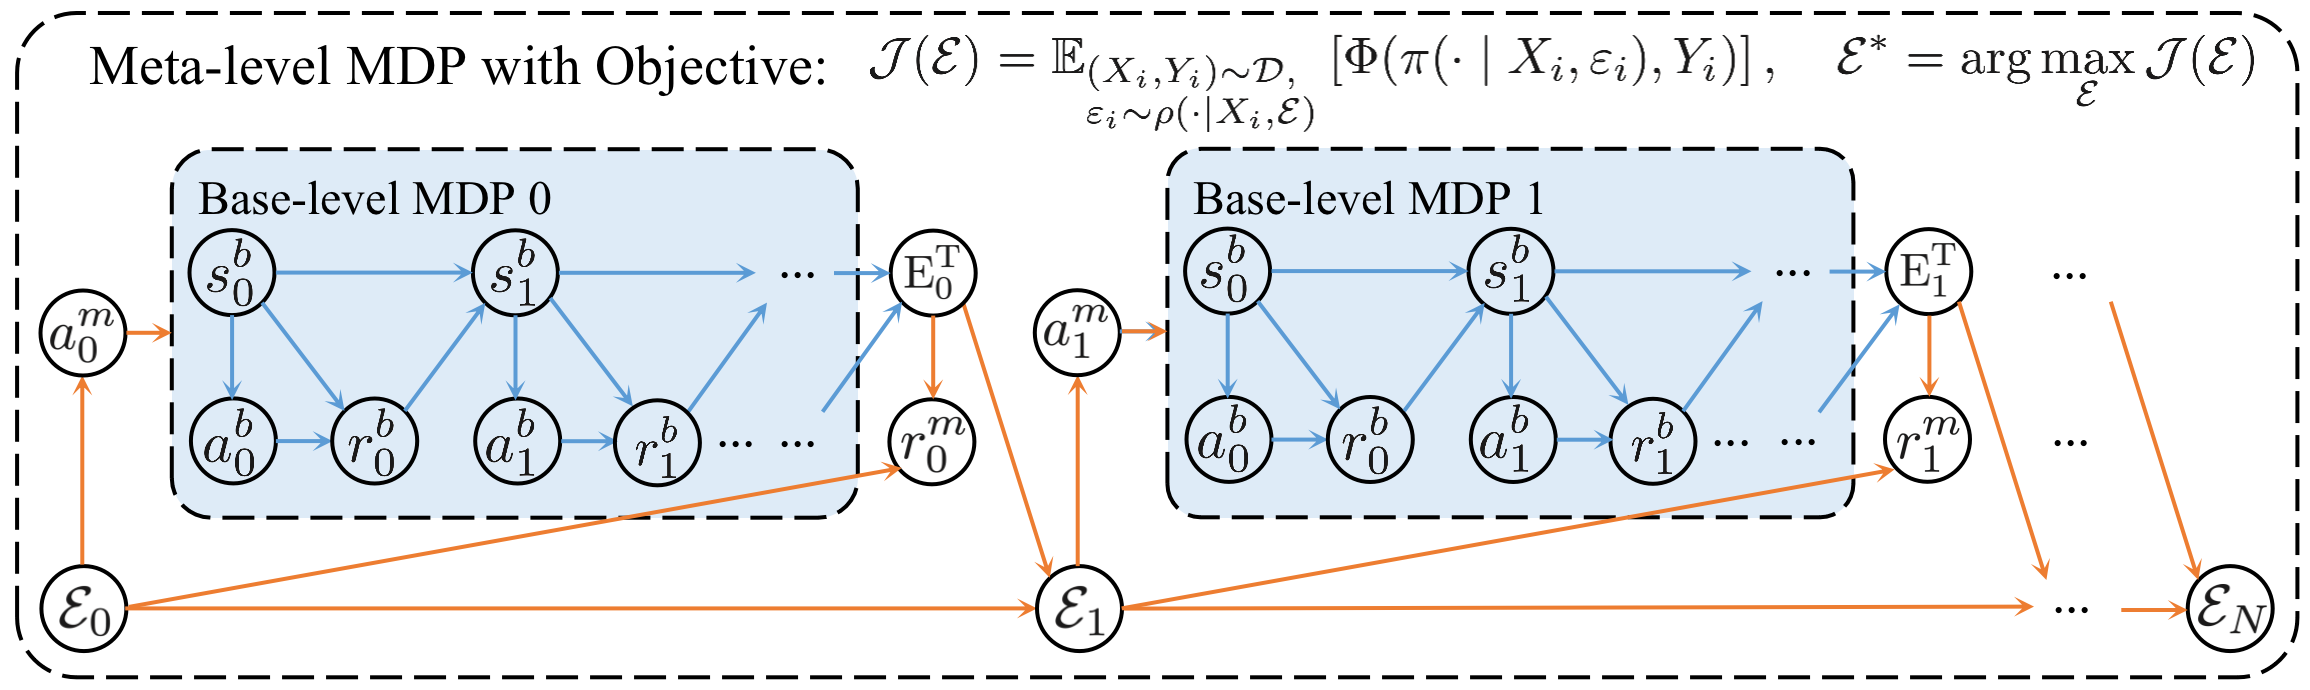
\includegraphics[width=0.98\linewidth]{./figs/fig-mdp.png}
  \caption{Illustration of the Meta-MDP formulation of \method{}.
The Base-level MDP performs intra-sample exploration and experience distillation, while the Meta-level MDP integrates these experiences to evolve the global experience library through forward updates.}
  \label{fig:mdp}
\end{figure}

\subsection{Optimize \method{} as Meta-MDP}
Unlike conventional gradient-based optimization, \method{} adopts a forward, experience-driven semantic evolution paradigm. 
Since the update rule of \method{} in Definition 2 produces an updated experience library that depends solely on the current state and is independent of historical states, we can formalize the optimization procedure as a hierarchical Meta Markov Decision Process (Meta-MDP) as shown in Fig~\ref{fig:mdp}, comprising Base-level MDPs that explores extensive experience, and a Meta-level MDP that governs the experience library evolution, enabling forwardly learning from accumulated experience instead of gradient back-propagation.

\paragraph{Meta-level MDP for Experience Library Evolution}
\begin{definition}[Meta-level MDP for Experience Library Evolution]
The Meta-level MDP is formally defined as the tuple $(\mathcal{S}^{m}, \mathcal{A}^{m}, \mathcal{T}^{m}, \mathcal{R}^{m})$:
\begin{itemize}
    \item \textbf{Meta-state} $s^{m}_i$: The current experience library $\mathcal{E}_i$
    \item \textbf{Meta-action} $a^{m}_i = \Psi({E^T_i}\mid X_i,Y_i,\mathcal{E}_i)$: Invokes the Base-level MDP on sample $(X_i,Y_i)$ under $\mathcal{E}_i$, yielding explored experiences ${E^T_i}$
    \item \textbf{Transition function} $\mathcal{T}^{m}$: Conducted by the updater $\mu$, evolves the experience library as $\mathcal{E}_{i+1}\sim\mathcal{T}^{m}(\mathcal{E}_{i+1}\mid \mathcal{E}_i,{E^T_i})$ under the meta-policy
    \item \textbf{Reward} $r^{m}_i = \Phi\big(\pi(\cdot\mid X_i, \rho(\cdot\mid X_i,\mathcal{E}_{i+1})),Y_i\big)$: Measures correctness of model output given $\mathcal{E}_{i+1}$
\end{itemize}
\end{definition}

Consequently, the cumulative return $G^{m} = \sum_{i=0}^{N-1} r^{m}_i$ over one meta-episode reflects the aggregated model accuracy across all $N$ training samples.
Therefore, maximizing $G^{m}$ is essentially equivalent to optimizing the objective in Eq.~\ref{eq:obj}.

In summary, this Meta-level formulation establishes a higher-order optimization loop that continuously refines the experience library through forward experiential updates, orchestrating Base-level exploration with long-term performance optimization.


\paragraph{Base-level MDP for Extensive Experiences Exploration} 
The Base-level MDP operationalizes the exploratory component of \method{} with an actor–critic framework. The actor iteratively generates diverse reasoning trajectories, while the critic provides semantic feedback that reflects on these trajectories, distilling them into structured experiences for Meta-level optimization, thus can be formulated as,
\begin{definition}[Base-level MDP for Experience Exploration]
The Base-level MDP is formally defined as the tuple $(\mathcal{S}^{b}, \mathcal{A}^{b}, \mathcal{T}^{b}, \mathcal{R}^{b})$:
\begin{itemize}
    \item \textbf{Base-state} $s^{b}_t$: The accumulated experience ${E^t_i}$ derived from the first $t$ reasoning trajectories explored on $X_i$ given $\mathcal{E}_i$
    \item \textbf{Base-action} $a^{b}_{t}$: One complete reasoning trajectory proposed by the actor $\pi$
    \item \textbf{Base-reward} $r^{b}_{t}=\Gamma(a^{b}_t,Y_i)$: Semantic feedback distilled by the critic, evaluating both the reasoning process and outcome relative to $Y_i$, capturing success patterns and interpretative insights
    \item \textbf{Transition function} $\mathcal{T}^{b}$: Updates the intra-sample experience accumulation as $s^{b}_{t+1} \sim \mathcal{T}^{b}(s^{b}_{t+1}\mid s^{b}_{t},r^{b}_{t})$, progressively integrating reflective knowledge until exploration terminates.
\end{itemize}
\end{definition}

Upon completion, the accumulated experience $E^T_i = s^{b}_T$ is returned to the Meta-level MDP for high-level experience library evolution.

Together, the Base-level and Meta-level MDPs form a hierarchical, closed-loop optimization process, the Base-level conducts fine-grained exploration and reflection within individual samples, while the Meta-level integrates these experiences across samples to continuously evolve the experience library in a gradient-free, forward-learning manner.


\section{Concrete Instantiation of \method{}}


Building on the mathematical formulation, we instantiate \method{} as a concrete mechanism consisting of two core components, namely, extensive experience exploration via the actor–critic forward loop and experience library evolution that consolidates and reuses experiential semantics.
Together, these two components realize continual semantic evolution through structured experience interaction as shown in Fig~\ref{fig:fl}.

\subsection{Extensive Experience Exploration}
The generation and collection of experiences are realized through per-case actor–critic interactions defined by the Base-level MDP. The key objective is to perform extensive exploration while ensuring that the collected experiences are both diverse and semantically informative.

\paragraph{Extensive Exploration Mechanism.}
To enable extensive high-quality exploration, we design a dual-scaling mechanism that combines parallel and sequential scaling. 
For \emph{parallel scaling}, multiple reasoning trajectories are sampled in parallel for the same input through rejection sampling~\cite{fujimoto2021minimalist,dong2023raft,gulcehre2023reinforced}, allowing diverse reasoning hypotheses to be explored and high-quality outputs to be retained.
For \emph{sequential scaling}, the actor iteratively improves upon its previous output under the critic’s semantic feedback~\cite{yuksekgonul2024textgrad,shinn2023reflexion}, where the critic provides constructive guidance and refinement cues derived from the prior round.
This cooperative exploration strategy balances breadth and depth, ensuring both coverage of alternative reasoning paths and progressive improvement over iterations.

\paragraph{Iterative Refinement with Semantic Signal.}
To ensure that collected experiences contribute meaningfully to learning, we design an iterative refinement mechanism driven by semantic evaluation.
For reasoning trajectories that lead to incorrect conclusions, the critic first identifies the underlying causes of failure and summarizes them into abstract, task-agnostic improvement suggestions.
These generalized feedback signals, denoted as new experiences $E_t$, are fed back into the actor together with its previous reasoning trace to initiate the next actor–critic iteration.
This process continues until the actor produces a correct or sufficiently improved reasoning trajectory, or a predefined iteration limit is reached.
In this loop, the critic’s feedback functions as a \emph{semantic update signal}~\cite{yuksekgonul2024textgrad,shinn2023reflexion,madaan2023self} that guides the actor’s reasoning refinement, analogous to the gradient signal in traditional optimization, yet expressed in natural language semantics rather than numerical differentials.
Unlike backpropagation-based learning, which relies on scalar gradients with limited interpretive bandwidth and heavy computational budget, this forward semantic feedback mechanism provides rich interpretable guidance without costly parameter updating, aligning with the cognitive characteristics of \textit{human-like learning from experience}.

Once the iterative refinement completes, validated experiences are distilled and passed to the Meta-level MDP, evolving experience library for long-term accumulation.

\begin{figure}[!t]
  \centering
  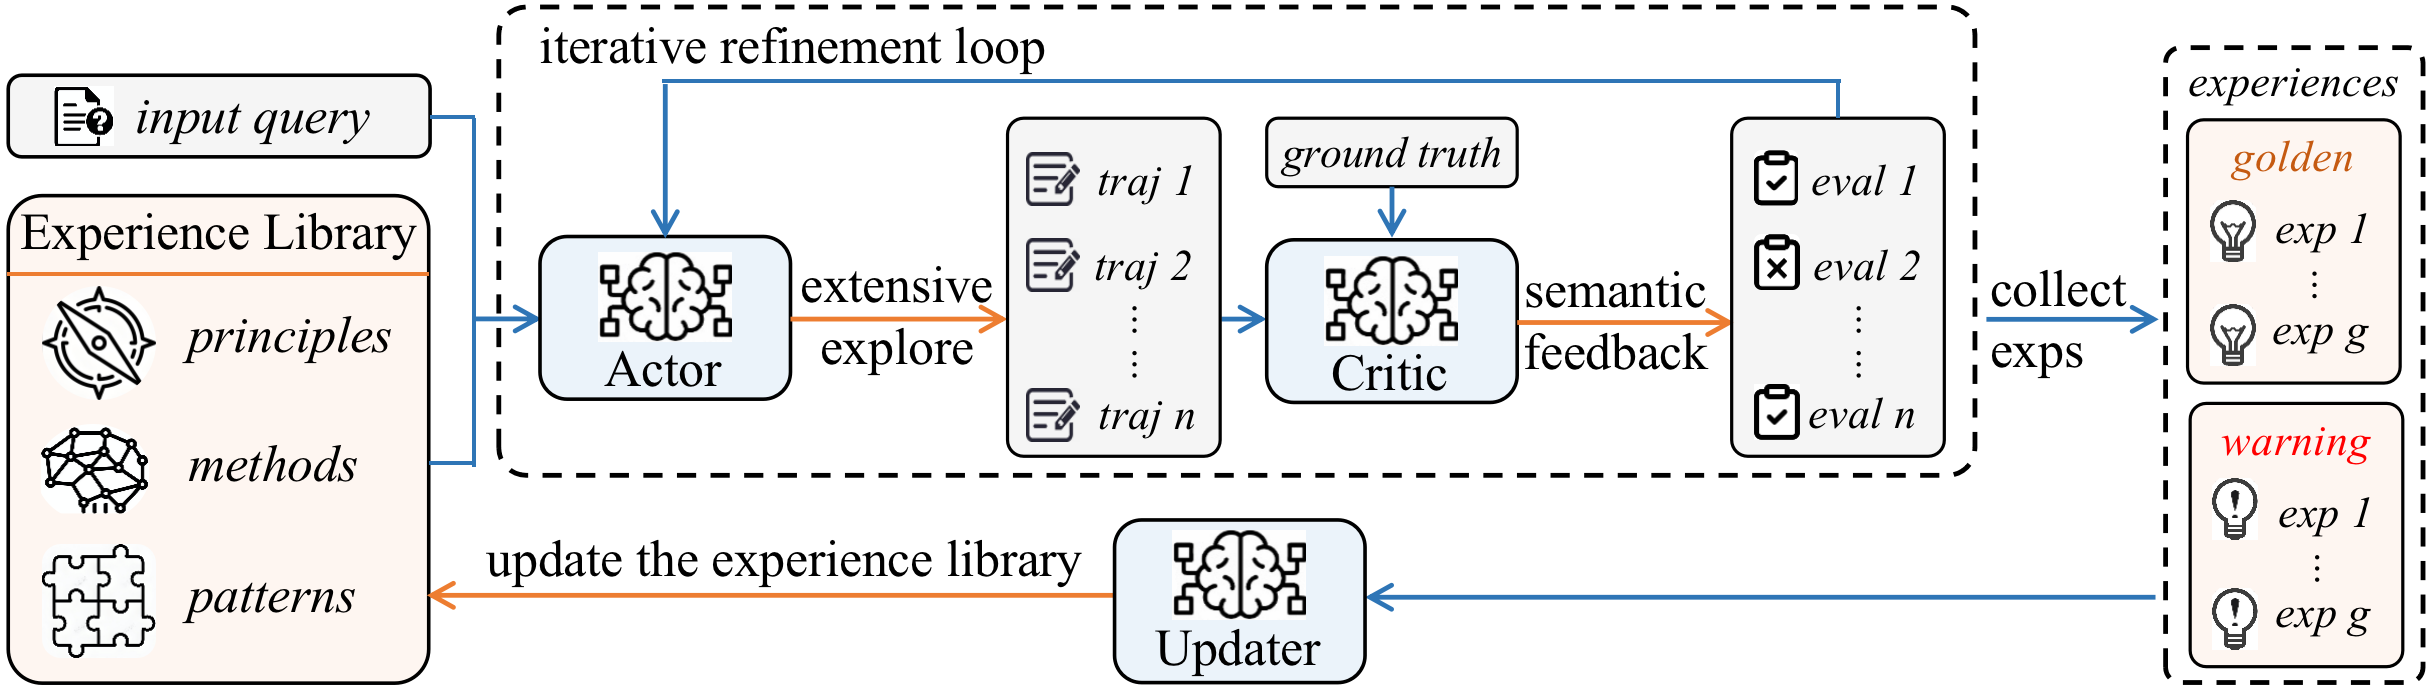
\includegraphics[width=0.98\linewidth]{./figs/fig-fl.png}
  \caption{Concrete Instantiation of \method{}. The refinement loop of actor-critic iteratively explores and refines experiences, then the meta-level updater dynamically organizes the distilled experiences into the evolving experience library.}
  \label{fig:fl}
\end{figure}
\subsection{Experience Library Evolution}
The experience library is hierarchically organized and continually evolves within the Meta-level MDP formulated above, driven by two complementary operations, update and retrieval, which together constitute the core meta-level transition dynamics.

\paragraph{Hierarchical Experience Library.}
The experience library adopts an explicit textual storage mechanism, which enables explicit recording of experiential rules, externalization of internal reasoning behaviors, and visualization of the learning dynamics, thereby enhancing interpretability and transparency.
To effectively organize learned experiences varying in granularity, abstraction, and contextual dependency, we design a hierarchical organization mechanism with three interconnected levels, namely, high-level strategic principles and guidelines, mid-level reasoning patterns and methodological templates, and low-level factual knowledge and concrete instances.
In addition, the library is partitioned into two complementary zones: the \textit{golden} zone, which stores experiences distilled from correct reasoning trajectories, and the \textit{warning} zone, which records failure cases and diagnostic insights extracted from erroneous trajectories.
Such dual-zone organization facilitates balanced learning from both successes and failures, allowing the agent to not only consolidate validated reasoning paths but also internalize the lessons encoded in previous mistakes.
This structure allows experiences to be modularly indexed and retrieved across abstraction levels, enabling both top-down guidance and bottom-up consolidation of knowledge.
Hierarchical organization also supports dynamic restructuring as new experiences are incorporated, maintaining the coherence of the library during continual evolution.
%In the future, we will explore more efficient yet interpretable storage mechanisms and more expressive hierarchical structures.

\paragraph{Experience Update Mechanism.}
Given a newly generated experience $\varepsilon$, the \textbf{updater} agent autonomously decides whether and how to incorporate it into the experience library. 
If an identical entry already exists, $\varepsilon$ is discarded to maintain compactness. 
If semantically similar entries are found, the agent performs a selective merge, preserving the more informative or higher-quality trajectory while minimizing redundancy. 
Otherwise, $\varepsilon$ is inserted into the appropriate partition and hierarchical level according to its semantic granularity. 
This adaptive update process ensures that the experience library incrementally evolves toward a more structured and informative representation of accumulated knowledge, rather than expanding indiscriminately or degenerating into redundant memory accumulation.

\paragraph{Experience Retrieval Mechanism.}
During inference, the experience library is encapsulated as an interactive \textbf{tool} callable by the agent~\cite{yao2022react,qiu2025alita}.
Instead of static vector-based semantic-similarity search~\cite{reimers2019sentence,ram2023context,karpukhin2020dense}, the agent performs contextualized retrieval conditioned on the specific query and its current reasoning state. 
This allows the agent to interpret relevance not only by semantic similarity but also by contextual consistency and goal alignment, thereby avoiding the pitfalls of retrieving semantically similar yet pragmatically contradictory entries.
Retrieval proceeds hierarchically, the agent first identifies relevant high-level strategies, then locates corresponding procedural patterns, and finally accesses concrete case examples within each pattern. 
At each stage, the top-$k$ (typically $k=5$) most relevant entries are selected to balance precision and efficiency. 
The retrieved experiences support the agent’s ongoing reasoning, reflective self-evaluation, and corrective refinement.
Moreover, retrieval is not restricted to pre-inference access, instead, the agent can dynamically query the library during reasoning, enabling adaptive integration of prior knowledge into evolving cognitive trajectories.

Overall, the update–retrieval dynamics establish a self-organizing experiential system that progressively refines its hierarchical organization and semantic granularity, facilitating the agent’s continual evolution through accumulated experience.